\section{Functionality description} \label{sec:functionality_description}
In this section the overall functions and the different parts of the \projname{} are described. The fully built \projname{} includes four sensors and four servo motors, which means that it also includes two NXT bricks, as it only supports three outputs per brick for the motors. The robot drives in the environment, using the interactive servo motor until it locates an object, using the ultrasonic sensor, or the black boundary using the colour sensor. If it locates an object, the master brick transmit a signal to the slave brick to commence the collection task. During this time, the robot stands still, waiting on a signal. All the components and how they are connected to the NXT bricks are shown in \figref{fig:robot_overview}. 

\subsection{Brick communication}
The two NXT bricks used for the robot is required to communicate in order to start and stop certain tasks. The integrated Bluetooth is used for communication between the NXT bricks. One of the two NXT bricks is chosen to be the master and the other one is the slave. The master unit controls the primary task of the robot, while the slave is used to handle a smaller, parallel task when receiving instructions from the master unit. 

\subsection{Colour sensor} 
The robot is equipped with two colour sensors on the front of the robot, one at each side. This is used to detect the black lines that specify the boundary of the environment. Based on the returned light the colour sensors return the RGB value to the NXT brick. The two colour sensors are handled by the master unit. 

\subsection{Ultrasonic sensor}
The ultrasonic sensor is placed in the front of the robot, just under the claw. This is used to detect the distance to the objects in front of the robot. The master unit is controlling the ultrasonic sensor.

\subsection{Compass sensor}
The compass sensor is placed on the top or the robot, at the end of an arm, so that it is located as far from the bricks and motors as possible. This is to reduce the noise from the magnetics fields created by these components. The sensor is pointing in the same direction as the robot. The compass sensor is used to help ensure precision in the robots movement. This increased precision in movement is used when searching for objects.

\subsection{Interactive servo motor}
The four interactive servo motors is used for two tasks. The first task is to move the robot around the environment. This includes driving forward, backward, and turning. The second task is the arm and the claw. This task consist of squeezing the claw around a detected object and holding this until the arm has reached the point, where the claw can let go of the object, and this lands in the storage behind the robot. Then the arm returns to the starting position, ready to grab a hold of new objects. Both task use 2 motors. The driving task is handled by the master unit, and the collection task is handled by the slave unit.

\subsection{Motor controller}\label{sec:design-motor-controller}
The tests in \secref{sec:servo_motor} proves that the motors used in the project are not very precise. It was decided to implement a motor controller to solve the precision issues. The objective for the motor controller is to ensure that the movement motors reach the same distance at the same time. 

The motor controller has two goals: reaching the destination, and ensuring that the motors has driven the same amount of steps. 

The left motor is selected as the motor where the speed is changed, and the right motor moves at constant speed. Based on how many steps each motor has turned at any given time and the moving direction, the speed is increased or decreased on the left motor. The motor controller ensures that the robot stops at the targeted number of steps $+/-$ an acceptable error margin.

It is not possible to make the motors 100\% precise, because the speed required to drive the robot is too high for it to be possible to make accurate calculations with it. This minimal speed is required due to the weight of the robot. To deal with this problem, a reasonable error margin is chosen. 

The result of the controller is a robot that, even though the hardware is imprecise, moves straight and behaves as expected.

\begin{figure}[H]
     \center{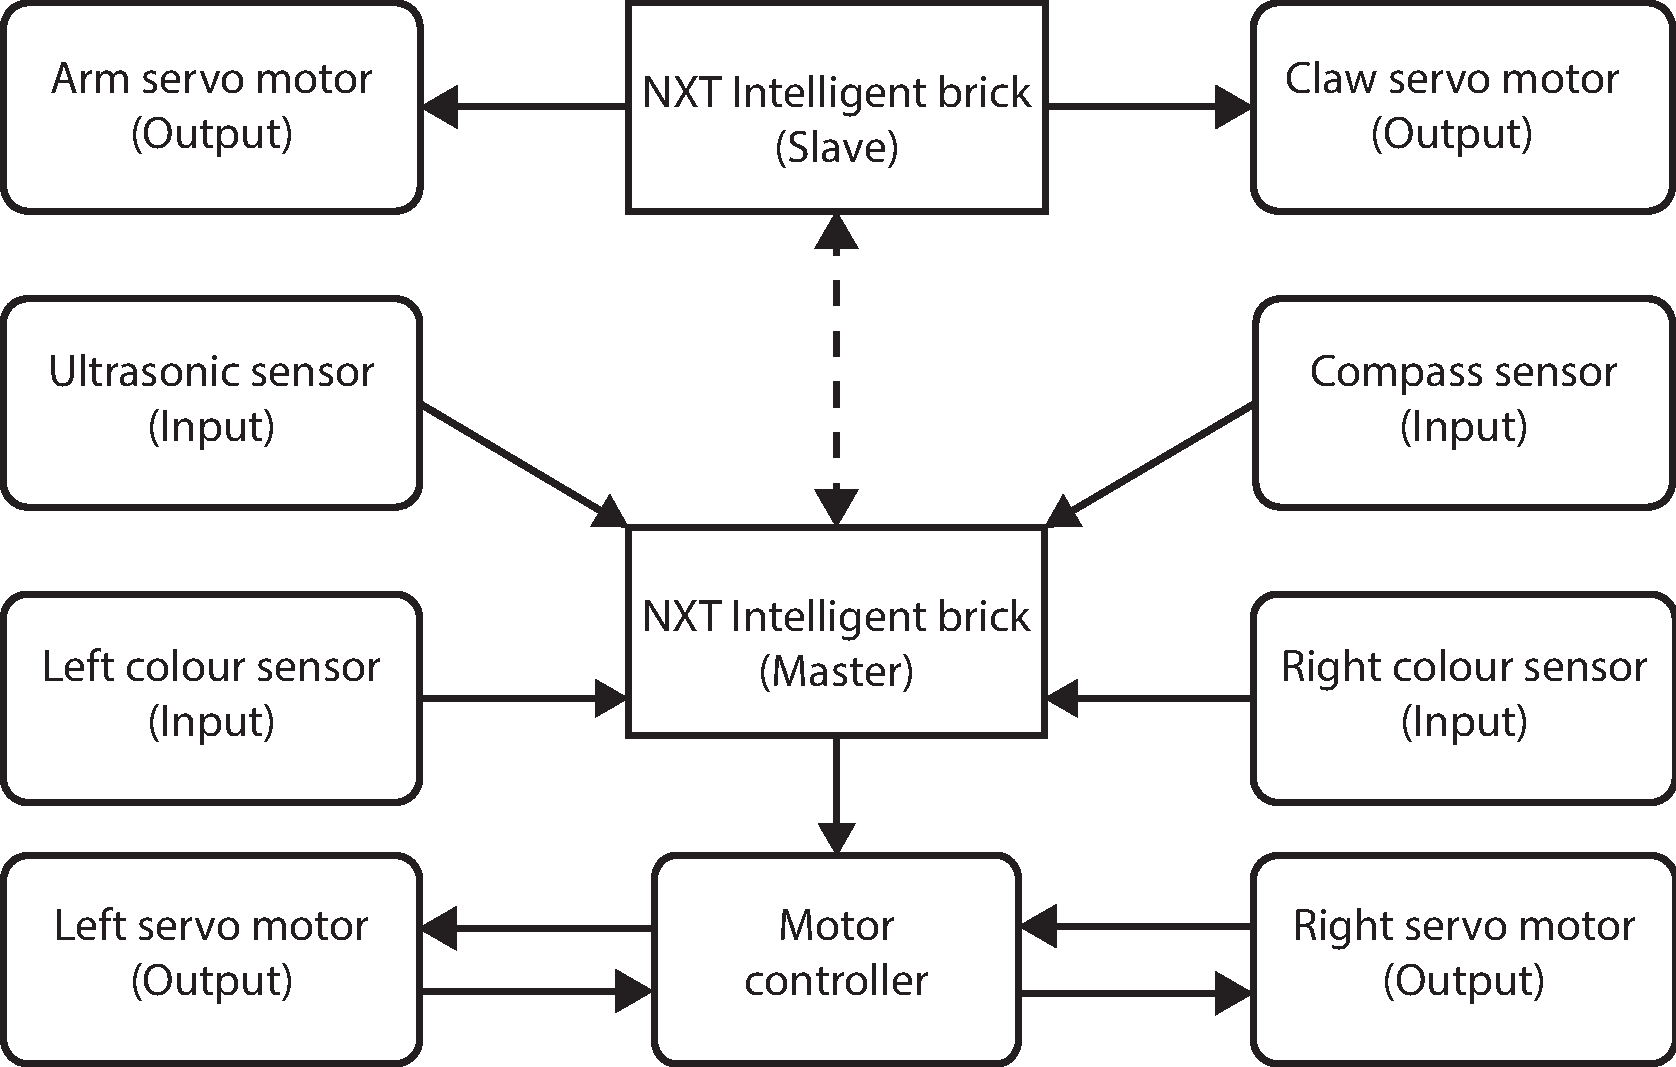
\includegraphics[width=\textwidth]
     {graphics/ComponentDiagram.pdf}}
     \caption{\label{fig:robot_overview} Diagram of all the components included in the robot.}
\end{figure}

